\documentclass{article}

\usepackage{graphicx}

\begin{document}
 
\title{Evaluation of Timestamp Distortions by Diverging Clock Domains in HICANN V2}
\author{S. Scholze and J. Partzsch}
\maketitle

\section{Problem Description}

In the design of the HICANN, there are two PLL (phase locked loop) modules, that supply the chip with different clocks.
One PLL is used for the OCP protocol and full-custom core components and the other PLL supplies the layer 2 communication components.
In detail, the second PLL provides the 1GHz/500MHz communication clock and the internal 250MHz for protocol functionalities and also for global system time components.
As this PLL is also used in all DNCs and all other HICANNs for the global synchronization of the system time, the frequency cannot be configured and the system time counters are all realized by using this PLL in the system.
The capturing of the neural events in the HICANN in contrast is realized with the first PLL, that needs to be configurable in frequency.
This capturing also includes adding the current system time counter to the pulse event as a timestamp.
For this, the timestamp value of the global system time needs to cross the different clock domains.
At this take over, distortions in the captured timestamp may occur.
This is analysed in the following.

\section{Analysis Method}

We used the test mode tmag\_timestamptest to evaluate the above problem.
Within this test, pulses are generated at regular intervals by the background generators in the HICANN.
Timestamps for the pulses are generated in the HICANN, which are subject to the mentioned timestamp distortions.
Pulse packets with these timestamps are sent via DNC to the FPGA, where they are stored in a trace memory and read out to the host PC from there.
Additionally, the FPGA timestamp is registered with each pulse.

All timestamps of one experiment run are stored in a text file.
Analysis and plotting is performed with the Python script analyse\_timestamps.py, which can be found in the same directory as this document.
Usage is as follows:
\begin{verbatim}
python analyse_timestamps.py <datafile>
\end{verbatim}

The script displays three plots:
The first one shows the raw HICANN timestamps in the order they have been received.
The second one displays a histogram of the time differences between HICANN and FPGA.
Ideally, these values should be constant; any deviations in it reflect the timestamp distortions.
The third diagram shows the transformation of the deviations to a biological timescale for an acceleration factor of $10^4$.

\section{Results}

Tests have been performed for different clock frequencies of the HICANN core clock domain.
The principal results are similar for all tested frequencies (100MHz to 250MHz).

\begin{figure}
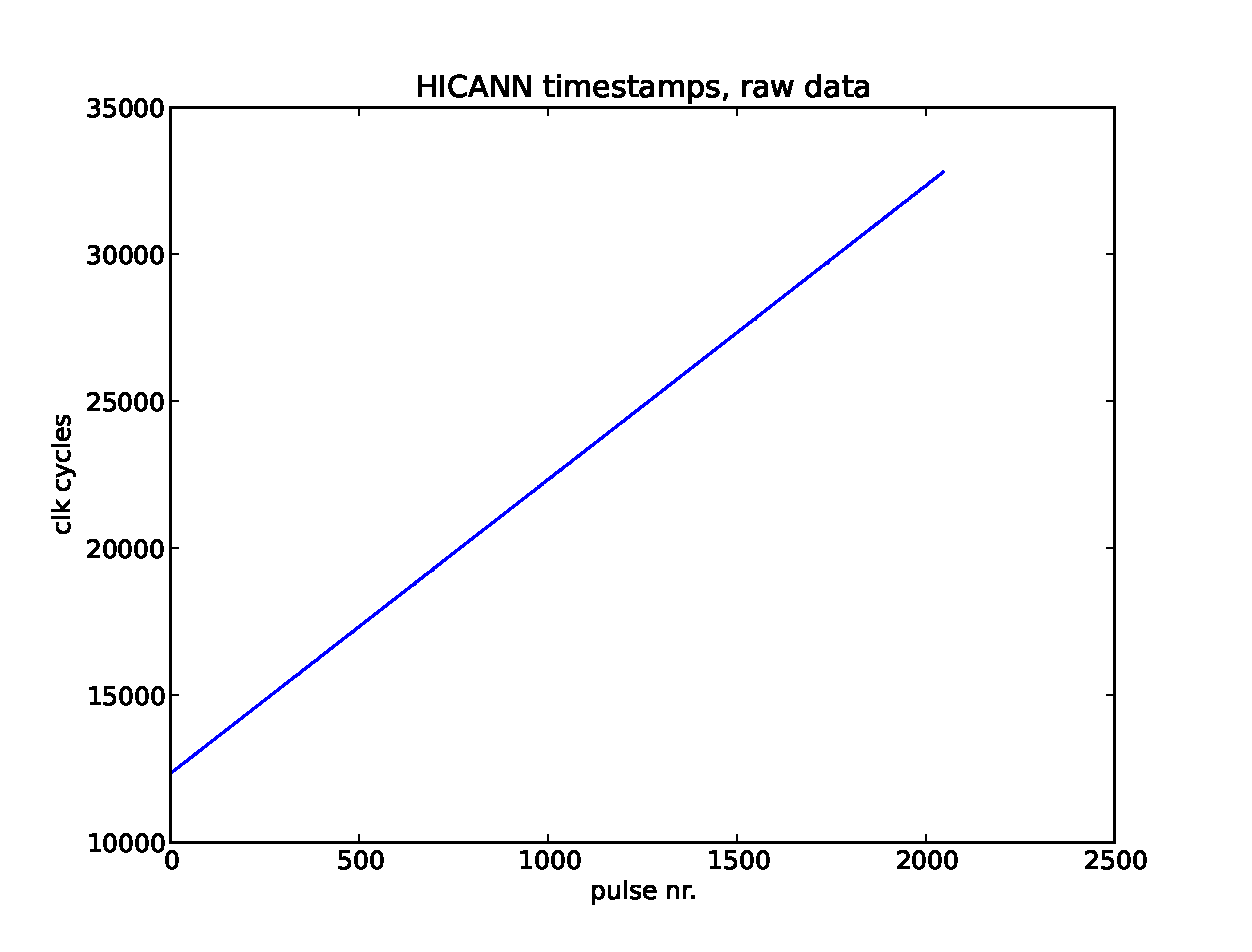
\includegraphics[width=0.32\textwidth ]{fig1_250mhz}
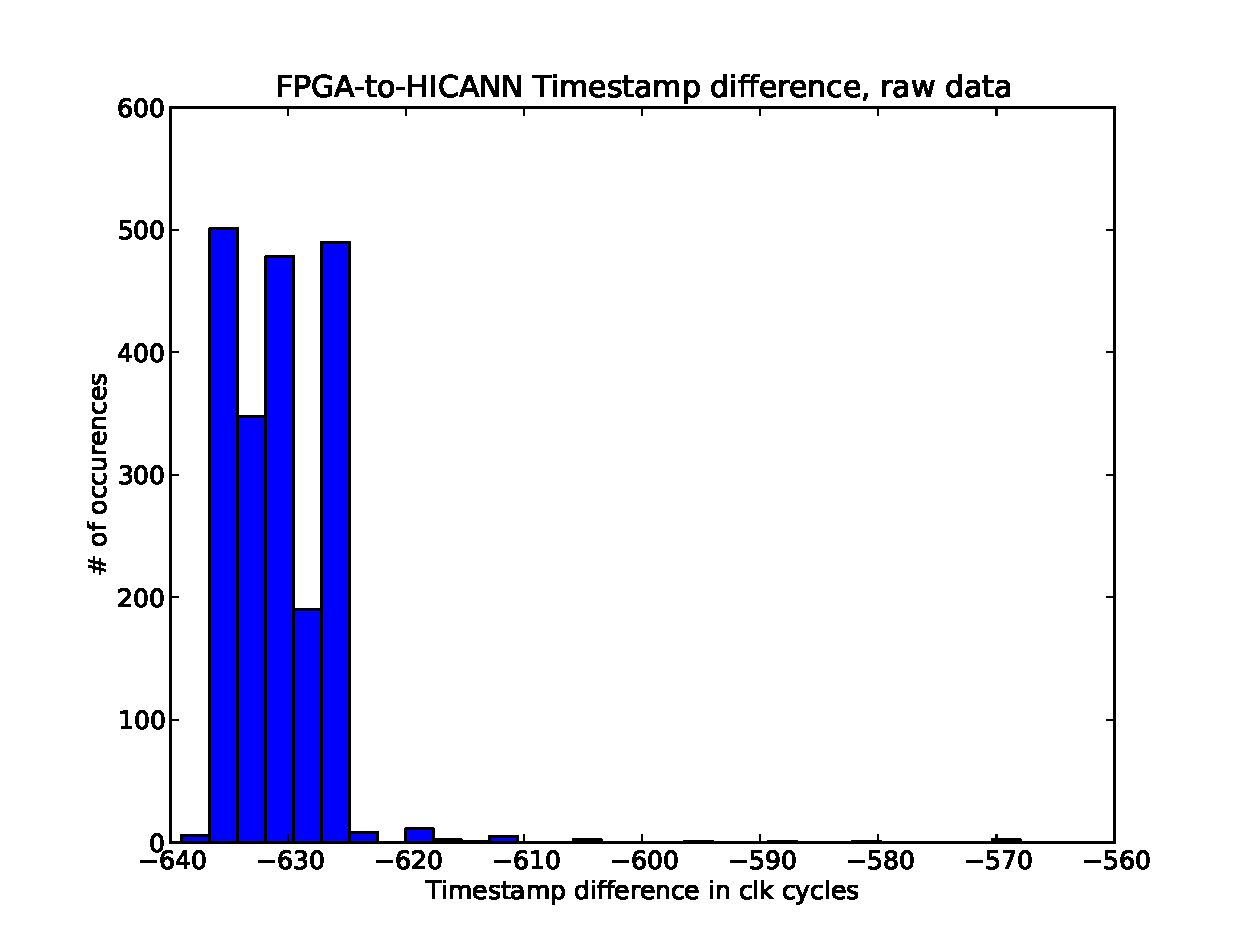
\includegraphics[width=0.32\textwidth ]{fig2_250mhz}
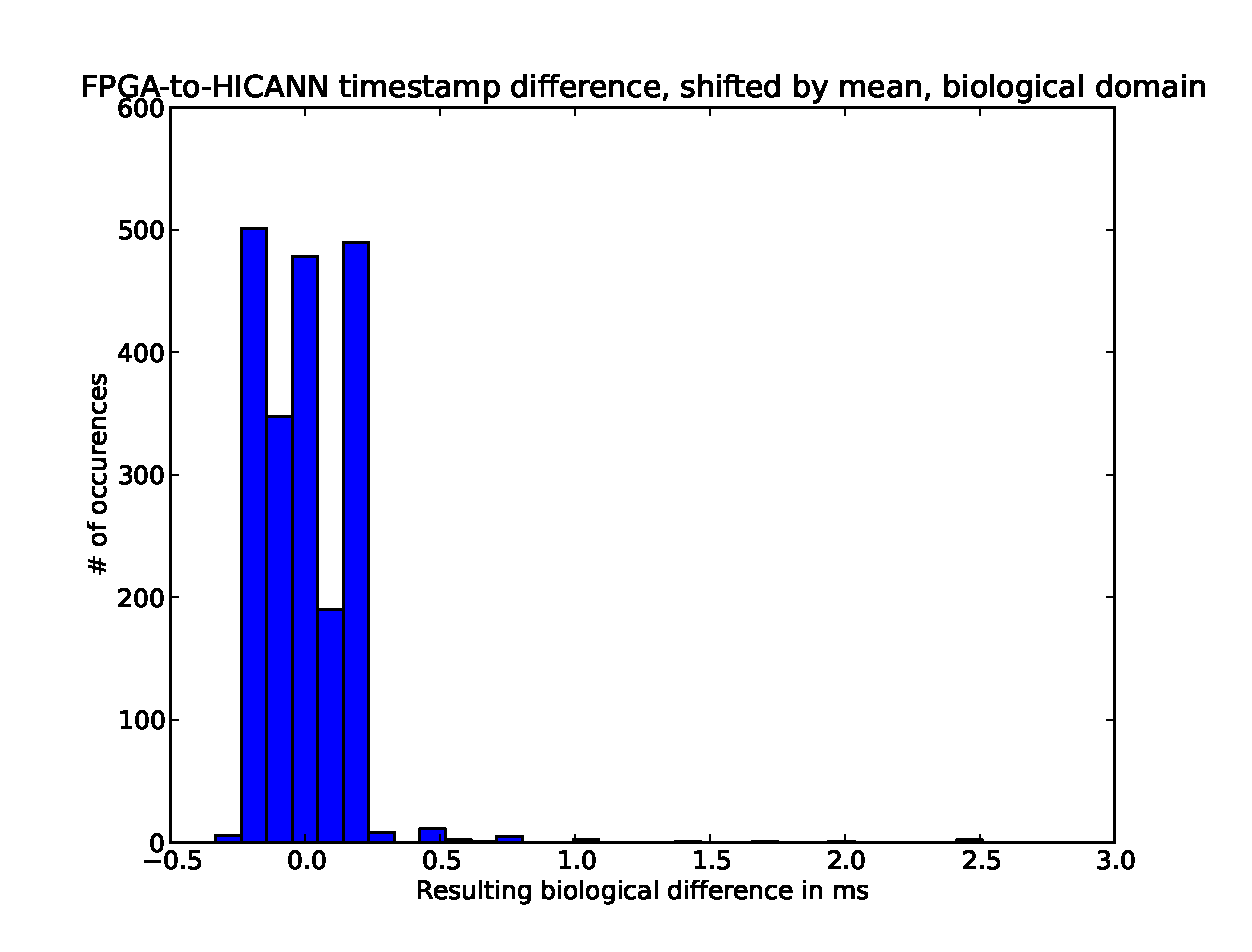
\includegraphics[width=0.32\textwidth ]{fig3_250mhz}
\caption{\label{fig_results} Results for a clock frequency of 250MHz.}
\end{figure}

Figure \ref{fig_results} shows the results for 250MHz core clock frequency.
In the raw timestamp differences between HICANN and FPGA, a systematic offset is present.
This is mainly due to the offset of the two timestamp counters, which results from the unsynchronized starting of these by the test mode.
If both counters were released synchronously, as is done in the final system, the offset would only reflect the transmission delay between HICANN and FPGA.

Most relevant for judging the impact of the timestamp distortions is the jitter of the timestamp difference.
For most pulses, this is in the order of some 100$\mu$s in the biological domain, reflected in the standard deviation of the time differences, which is 182$\mu$s in the shown case.
These values are within the time resolution of typical software simulations for spiking neural networks, which often use a fixed timestep of 100$\mu$s.
A small fraction of pulses ($<1$\%), however, shows deviations greater than 1ms, which may be more relevant for neuromorphic experiments.

In one case, we saw a complete cancelling of all bits in the HICANN timestamp, resulting in a single large deviation (see data provided for 100MHz).
As 10000 pulses were transmitted in all five tests, it can be assumed that the resulting large deviation occurs only very rarely.
Still, these cases can be easily corrected in the FPGA by comparing the received pulse timestamps from the HICANN with the FPGA system time counter. 

\end{document}
